\chapter{羧酸衍生物}\label{ch:b2:acyl-substitution}

用氢氧化钠煮沸橄榄油，即得到肥皂和甘油：这是
人类最早有意进行的有机反应。油脂是甘油与
长链酸形成的酯，氢氧根总在同一个键处将酯切开，
即羰基碳与醇基氧之间的键。酯、
酸、酰胺、酸酐和酰氯都以这种方式反应：亲核试剂
加成到羰基碳上，同时一个基团离去。将这些
化合物按其离去基团的能力排序，即可判断哪种可以转化为哪种，
以及化学家必须朝哪个方向“逆势而上”。

\begin{recall}
本科一年级分册：羰基的亲电活化，半缩醛与缩醛的生成机理，有机镁加成，
氢负离子供体及其适用范围，离去基团，
$\mathrm pK_a$、$Q$ 和 $K$。\Cref{ch:b2:amines}：亲核加成，胺。
\Cref{ch:b2:equilibrium-shifts}：平衡移动。第 1 册：酯、羧酸
与酰胺。
\end{recall}

\begin{omfigure}
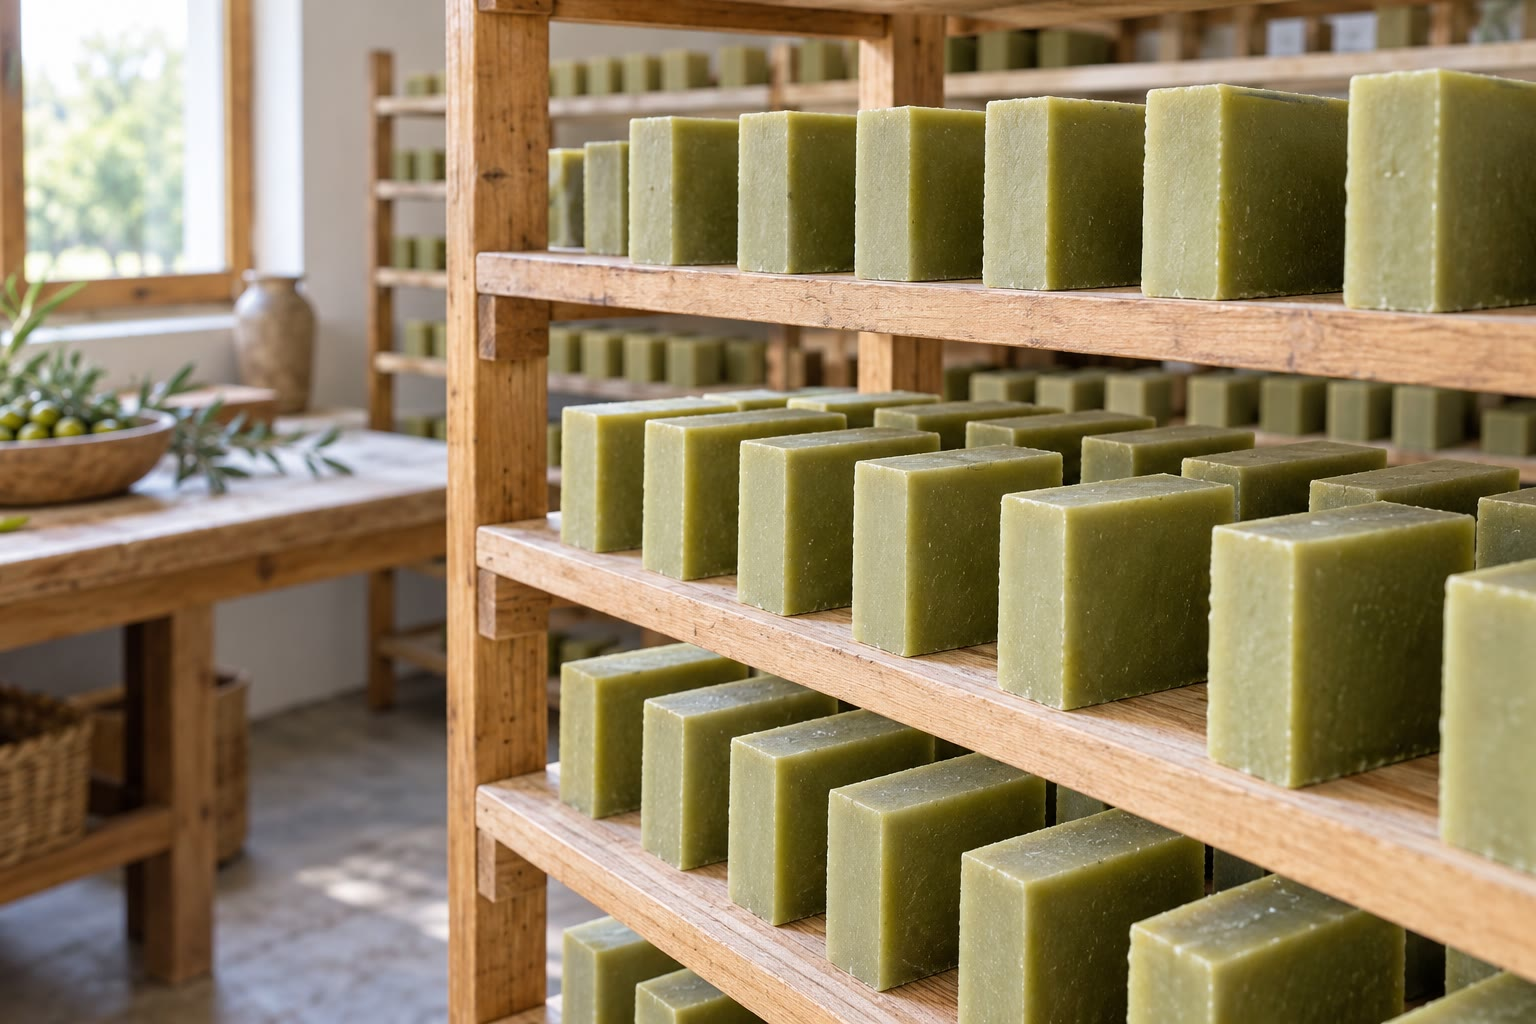
\includegraphics[width=0.58\linewidth]{images/book3/ai/b2-24-soap-bars.jpg}

{\small 晾在木架上的橄榄油皂条。肥皂是脂肪酸的钠盐，
这些脂肪酸在油（一种酯）与氢氧化钠共煮时释放出来。}
\end{omfigure}

\section{家族及其反应性}

\begin{definition}[羧酸衍生物]\label{def:b2:acyl-substitution:derivative}
称化合物 \ce{R-CO-Z} 为\emph{羧酸衍生物}\index{羧酸衍生物}，其中
羧酸的 \ce{OH} 被另一基团 Z 取代。所有衍生物共有的\emph{酰基}\index{酰基}
$\mathrm{R{-}CO{-}}$，在\emph{酰氯}\index{酰氯}中，
Z 为 Cl；在\emph{酸酐}\index{酸酐}中，Z 为 $\mathrm{O{-}CO{-}R'}$，两个酰基
共用一个氧原子；在酯中 Z 为 $\mathrm{OR'}$，在酰胺中为 $\mathrm{NR'_2}$。
\end{definition}

\begin{proposition}[反应活性顺序]\label{prop:b2:acyl-substitution:reactivity}
对亲核试剂而言，各衍生物的反应活性顺序为：酰氯 $>$ 酸酐 $>$ 酯
$\approx$ 羧酸 $>$ 酰胺。
\end{proposition}

\begin{proof}[论证]
两种效应叠加。离去基团 \ce{Z-} 的碱性越弱，越容易离去：
\ce{Cl-}（共轭酸为 \ce{HCl}，$\mathrm pK_a$ 约为 $-7$）远优于羧酸根
（$\mathrm pK_a$ 约为 5）、醇盐（约 16）或酰胺离子（约 35）。另外，基团 Z 借助其孤对电子的共振给电子作用，
向羰基供给电子密度，使羰基碳
的亲电性降低：对 Cl 较弱，对氮最强。酰胺既是
亲电性最差的衍生物，也是最差的离去基团。
% ledger: pka:ethanoic, pka:ethanol
\end{proof}

\section{亲核酰基取代}

\begin{definition}[亲核酰基取代]\label{def:b2:acyl-substitution:nas}
\emph{亲核酰基取代}\index{亲核酰基取代}是指以亲核试剂取代酰基化合物中的
基团 Z 的反应。其过程是亲核试剂加成到羰基碳上，
生成\emph{四面体中间体}\index{四面体中间体}，随后
离去基团脱去，恢复 \ce{C=O} 键。
\end{definition}

\begin{proposition}[加成–消除]\label{prop:b2:acyl-substitution:addition-elimination}
酰基取代经由四面体中间体进行；在碱性条件下，较强的亲核试剂使反应加快，
在酸性条件下，羰基的活化同样使反应加快。
\end{proposition}

\begin{proof}[论证]
羰基碳为平面结构、具有亲电性，亲核试剂可从平面上方或下方进攻，
与\cref{ch:b2:amines}中的加成相同；若基团 Z 能够离去，
中间体便将其排出，而不是被质子化。在碱性条件下，亲核试剂为阴离子（\ce{HO-}、
\ce{RO-}）；在酸性条件下，羰基氧被质子化，中性亲核试剂（水、醇）即可反应。
醇部分带 \ce{^{18}O} 标记的酯水解后，
得到带标记的醇和不带标记的酸：断裂的是酰基–氧键，这与机理相符。
\end{proof}

\begin{omfigure}
\setchemfig{atom sep=1.7em}
\schemestart
\chemfig{R-C(=[2]O)-OR'} \+ \chemfig{HO^{-}}
\arrow{->[加成]}
\chemfig{R-C(-[2]O^{-})(-[6]OH)-OR'}
\arrow{->[消除]}[,1.3]
\chemfig{R-C(=[2]O)-OH} \+ \chemfig{^{-}OR'}
\schemestop

\medskip
\schemestart
\chemfig{R-C(=[2]O)-OH} \+ \chemfig{^{-}OR'}
\arrow{->[质子转移]}
\chemfig{R-C(=[2]O)-O^{-}} \+ \chemfig{HOR'}
\schemestop
\par\vspace{6pt}

{\small 酯的皂化。氢氧根加成到羰基碳上，生成四面体中间体；
醇盐离去，\ce{C=O} 键重新形成；醇盐为强碱，随即夺取酸的质子。
最后一步使反应进行到底。}
\end{omfigure}

\begin{method}[画出酰基取代的机理]\label{met:b2:acyl-substitution:nas-mechanism}
\begin{enumerate}
  \item 碱性条件下：阴离子亲核试剂加成到羰基碳上，负电荷转移到
        氧原子上；\ce{C=O} 键重新形成，Z 离去；最后完成任意酸碱步骤。
  \item 酸性条件下：羰基氧质子化，中性亲核试剂加成，质子转移
        到离去基团上，离去基团以中性分子离去，最后羰基脱去质子。
  \item 清点步骤：每个中间体或为四面体型，或为羰基化合物。
\end{enumerate}
\end{method}

\section{酯}

\begin{definition}[酯化]\label{def:b2:acyl-substitution:esterification}
\emph{酯化}\index{酯化}是指由羧酸（或更活泼的
衍生物）与醇生成酯的反应。羧酸与醇在强酸催化下的直接反应，
即费歇尔酯化。
\end{definition}

\begin{proposition}[费歇尔酯化]\label{prop:b2:acyl-substitution:fischer}
费歇尔酯化是一个慢平衡，伯醇情形下平衡常数接近 4；
通过使某一反应物过量，或随生成随移除水，可使其正向进行。
\end{proposition}

\begin{proof}[论证]
等物质的量的乙醇与乙酸反应，当三分之二的酸被酯化时达到平衡：$K =
(2/3)^2/(1/3)^2 = 4$。若借助过量醇维持 $Q < K$，或将水蒸出
（本科一年级分册中的迪安–斯塔克分水器），反应将继续进行
（见\cref{ch:b2:equilibrium-shifts}）。该反应机理的六步与酸性条件下
\cref{met:b2:acyl-substitution:nas-mechanism}中的六步相同，均为可逆步骤。
% ledger: ester:berthelot
\end{proof}

\begin{definition}[皂化]\label{def:b2:acyl-substitution:saponification}
\emph{皂化}\index{皂化}是指酯被氢氧根水解，
生成羧酸盐和醇。
\end{definition}

\begin{proposition}[皂化反应进行到底]\label{prop:b2:acyl-substitution:saponification}
皂化反应进行到底：其最后一步为羧酸向醇盐的质子转移，
其平衡常数的量级为 $10^{11}$。
\end{proposition}

\begin{proof}
对于 $\mathrm{RCOOH + R'O^- \to RCOO^- + R'OH}$，
\[
  K = \frac{K_a(\ce{RCOOH})}{K_a(\mathrm{R'OH})} = 10^{\mathrm pK_a(\mathrm{R'OH}) - \mathrm pK_a(\ce{RCOOH})} ;
\]
乙酸（4.76）与乙醇（15.93）的情形下，$K = 10^{11.2}$。羧酸根是较差的亲电试剂，不会被醇进攻：
总反应不可逆。
% ledger: pka:ethanoic, pka:ethanol
\end{proof}

\begin{omfigure}
\setchemfig{atom sep=1.7em}
\schemestart
\chemfig{CH_2(-[0]O-CO-R)-[6]CH(-[0]O-CO-R)-[6]CH_2-[0]O-CO-R}
\+ \chemfig{3\,NaOH}
\arrow{->[加热]}
\chemfig{CH_2(-[0]OH)-[6]CH(-[0]OH)-[6]CH_2-[0]OH}
\+ \chemfig{3\,R-COO^{-}\,Na^{+}}
\schemestop
\par\vspace{6pt}

{\small 甘油三酯的皂化：三个酯键断开，生成甘油和
三分子羧酸钠，即肥皂（R 为长链，油酸根的 \ce{C17H33}
取自橄榄油）。}
\end{omfigure}

\begin{definition}[酯交换]\label{def:b2:acyl-substitution:transesterification}
\emph{酯交换}\index{酯交换}是指酯的醇部分发生交换，
即 $\mathrm{RCOOR' + R''OH \rightleftharpoons RCOOR'' + R'OH}$，在酸或碱催化下进行。
\end{definition}

\begin{definition}[内酯与内酰胺]\label{def:b2:acyl-substitution:lactone}
\emph{内酯}\index{内酯}是一种环状酯，由羟基酸
分子内酯化形成；\emph{内酰胺}\index{内酰胺}是一种环状酰胺。
\end{definition}

\section{活化衍生物}

沿活性序列向下转化较易：酰氯与合适的亲核试剂反应，可得酸酐、酯或
酰胺，通常在室温下即可进行。向上转化则需活化：
羧酸经亚硫酰氯转化为酰氯，
\[
  \ce{RCOOH + SOCl2 -> RCOCl + SO2 + HCl} ,
\]
其副产物均为气体。随后酰氯与醇或胺反应；加入碱
（吡啶、三乙胺，或另一当量的胺）以捕获生成的 \ce{HCl}，
否则它会使胺质子化。

\begin{method}[沿衍生物序列转化]\label{met:b2:acyl-substitution:ladder}
\begin{enumerate}
  \item 向下（氯化物 $\to$ 酸酐 $\to$ 酯，酸 $\to$ 酰胺）：用
        亲核试剂处理，并加入碱以吸收释放的酸。
  \item 向上：先将酸转化为酰氯（\ce{SOCl2}）；酯或酰胺需要
        先水解为酸。
  \item 酸与酯之间：费歇尔酯化（平衡）或皂化（完全）
        随后酸化。
\end{enumerate}
\end{method}

\begin{omfigure}
\begin{tikzpicture}[font=\small, >={Stealth}]
  \foreach \y/\n in {4/{酰氯 \ce{RCOCl}}, 3/{酸酐 \ce{(RCO)2O}}, 2/{酯 $\mathrm{RCOOR'}$ \quad 羧酸 \ce{RCOOH}}, 1/{酰胺 $\mathrm{RCONR'_2}$}} {
    \node[cyclenode, minimum width=5.2cm] at (0,\y*1.1) {\n};
  }
  \draw[->, thick, omDef] (-3.1,4.3) -- (-3.1,1.1) node[midway, left, align=right, font=\scriptsize] {容易：\\ 亲核试剂 \\ + 碱};
  \draw[->, thick, omThm] (3.1,2.2) -- (3.1,4.4) node[midway, right, align=left, font=\scriptsize] {上行：\\ 经羧酸 \\ 和 \ce{SOCl2}};
  \node[font=\scriptsize, anchor=south] at (0,4.85) {反应性更强};
  \node[font=\scriptsize, anchor=north] at (0,0.55) {反应性更弱};
\end{tikzpicture}

{\small 羧酸衍生物的活性序列。任一衍生物都可借助亲核试剂转化为
其下方的衍生物；向上则需经由羧酸及其酰氯。}
\end{omfigure}

\section{有机金属试剂与氢化物}

\begin{proposition}[两次格氏加成]\label{prop:b2:acyl-substitution:grignard-ester}
酯与过量的有机镁试剂反应，生成一种叔醇，
其上带有两个来自试剂的相同基团。
\end{proposition}

\begin{proof}[论证]
第一次加成生成四面体中间体，它消除醇盐而得到酮。酮
的亲电性比酯更强（$\mathrm{OR'}$ 基团无共轭给电子），与
试剂的反应比剩余的酯更快；第二次加成于酮上进行，生成
叔醇的醇盐，经酸后处理质子化。反应不能停留在酮这一步。
\end{proof}

\begin{proposition}[氢化物还原]\label{prop:b2:acyl-substitution:hydrides}
四氢铝锂可将酯和羧酸还原为伯醇，将酰胺还原为胺；
硼氢化钠可还原醛和酮，但不能还原酯、羧酸或酰胺。位阻较大的铝
氢化物（DIBAL-H）在 \qty{-78}{\degreeCelsius} 下可将酯还原为醛。
\end{proposition}

\begin{proof}[论证]
\ce{LiAlH4}为强氢负离子供体：与格氏试剂相似，它对酯加成两次（经由
醛）。硼氢化物对亲电性较弱的酯羰基而言太弱。低温下使用 DIBAL-H
时，四面体中间体由铝稳定，直到
水性后处理才消除醇盐，此时已无氢化物剩余，醛得以保留。在酰胺中，
与铝结合的氧而非氮被消除，留下一个亚胺离子，
它被氢化物还原为胺。
\end{proof}

\begin{history}[谢弗勒尔与油脂]
\begin{minipage}[t]{0.22\linewidth}
\vspace{0pt}
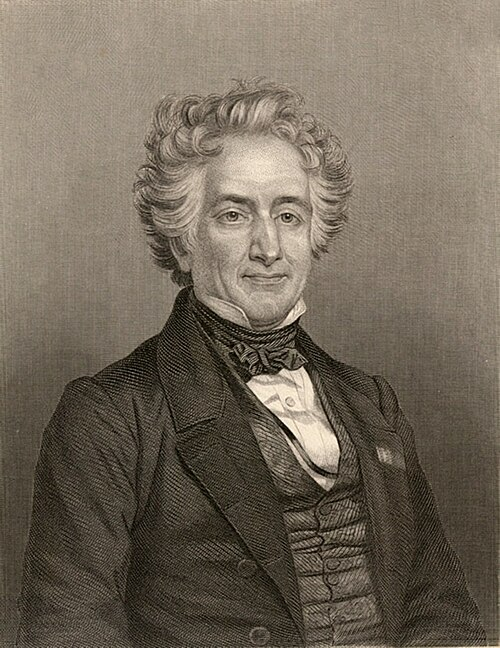
\includegraphics[width=\linewidth]{images/book3/chevreul.jpg}
\end{minipage}\hfill
\begin{minipage}[t]{0.74\linewidth}
\vspace{0pt}
米歇尔·欧仁·谢弗勒尔于 1823 年发表的研究中证明，油脂是甘油
与脂肪酸形成的化合物，他分离并命名了其中的脂肪酸（硬脂酸、油酸、丁酸），并证明
皂化可将它们分解为这两部分。他的工作使制皂与制烛成为化学研究的对象；
他活到了 102 岁。（肖像为尼古拉斯·欧斯塔什·莫兰所绘，公有领域，见维基共享资源
。）
\end{minipage}
\end{history}

\begin{safety}{\ghs[5mm]{GHS02}\,\ghs[5mm]{GHS05}\,\ghs[5mm]{GHS06}}
氯化亚砜和酰氯与水剧烈反应并释放腐蚀性气体；它们
须干燥操作，并在通风橱中进行。四氢铝锂遇水会着火；其
过量部分在最后小心销毁。浓氢氧化钠对皮肤和
眼睛具有腐蚀性。甲醇有毒且易燃。
% ledger: ghs:SOCl2, ghs:ethanoyl-chloride, ghs:LiAlH4, ghs:NaOH, ghs:methanol
\end{safety}

\section{练习}

\begin{exercise}[$\star$]\label{exo:b2:acyl-substitution:1}
按与水的反应活性排序：乙酸乙酯、乙酰氯、乙酰胺、乙酸
酐。
\end{exercise}

\begin{exercise}[$\star$]\label{exo:b2:acyl-substitution:2}
写出乙酰氯分别与下列物质反应的生成物：水；乙醇；氨（2 当量）；
乙酸钠；二甲胺并加入三乙胺。
\end{exercise}

\begin{exercise}[$\star$]\label{exo:b2:acyl-substitution:3}
写出苯甲酸甲酯与氢氧化钠发生皂化的反应式，并计算
\qty{13.6}{g} 该酯所需氢氧化钠的质量。
\end{exercise}

\begin{exercise}[$\star$]\label{exo:b2:acyl-substitution:4}
画出 4-羟基丁酸形成的内酯，并给出其环的大小。
\end{exercise}

\begin{exercise}[$\star\star$]\label{exo:b2:acyl-substitution:5}
写出乙酸乙酯与氨反应的反应机理。
\end{exercise}

\begin{exercise}[$\star\star$]\label{exo:b2:acyl-substitution:6}
阿司匹林由水杨酸（2-羟基苯甲酸）和乙酸酐制得。水杨酸中哪个
基团参与反应，副产物是什么？
\end{exercise}

\begin{exercise}[$\star\star$]\label{exo:b2:acyl-substitution:7}
乙酸乙酯与过量的甲基溴化镁反应，再用稀酸处理。写出
生成物，并解释为何无法分离得到酮。
\end{exercise}

\begin{exercise}[$\star\star$]\label{exo:b2:acyl-substitution:8}
写出练习 4 中内酯被 \ce{LiAlH4} 还原的生成物。
\end{exercise}

\begin{exercise}[$\star\star$]\label{exo:b2:acyl-substitution:9}
已知 $K = 4$，计算乙酸分别与一当量和三当量乙醇
发生酯化的比例。还有哪种方法可驱动反应？
\end{exercise}

\begin{exercise}[$\star\star\star$]\label{exo:b2:acyl-substitution:10}
以苯甲酸为原料制备 \textit{N},\textit{N}-二乙基苯甲酰胺，并解释为何将酸
与二乙胺混合后温和加热却生成一种盐。
\end{exercise}

\begin{exercise}[$\star\star\star$]\label{exo:b2:acyl-substitution:11}
油脂的皂化值是指皂化
\qty{1}{g} 油脂所需氢氧化钾的质量，单位为 mg。计算三油酸甘油酯的皂化值（\qty{885.4}{g/mol}；KOH \qty{56.11}{g/mol}）。
\end{exercise}

\begin{exercise}[$\star\star\star$]\label{exo:b2:acyl-substitution:12}
某分子同时含有酯基、酰胺基和酮基。哪些基团会被 \ce{NaBH4} 还原，哪些
会被 \ce{LiAlH4} 还原？各得到什么生成物？
\end{exercise}

\section{周末问题：由煎炸油制备生物柴油}

\begin{problem}[{周末问题——三油酸甘油酯及其摩尔质量、它与
甲醇的酯交换反应及碱的作用、与游离酸和水的副反应，以及每
吨油的产率}]
\label{pb:b2:acyl-substitution:1}
将油视为纯三油酸甘油酯，它是油酸（\ce{C17H33COOH}）的甘油三酯。摩尔质量
（\unit{g/mol}）：C 12.011，H 1.008，O 15.999，Na 22.990。甘油为丙-1,2,3-三醇。
% ledger: aw:C, aw:H, aw:O, aw:Na, ghs:methanol, ghs:NaOH

\medskip
\noindent\textbf{第一部分——三油酸甘油酯。}
\begin{enumerate}
  \item 写出油酸和甘油的化学式。
  \item 写出三油酸甘油酯的化学式，并计算其摩尔质量。
  \item 它含有几个酯基？
  \item 油酸含有一个顺式双键。为什么富含油酸的油脂在室温下为液体？
  \item 三油酸甘油酯皂化后会得到什么？
  \item 从化学角度看，生物柴油是什么？
\end{enumerate}

\medskip
\noindent\textbf{第二部分——酯交换。}
\begin{enumerate}[resume]
  \item 写出三油酸甘油酯与甲醇发生酯交换的反应。
  \item 为什么用碱（甲醇钠或氢氧化物）作催化剂？
  \item 画出第一步交换的四面体中间体。
  \item 为什么甲醇要过量使用（六当量而非三当量）？
  \item 甘油与甲酯不互溶，这对分离有什么帮助？
  \item 在理想反应中，催化剂是否被消耗？
\end{enumerate}

\medskip
\noindent\textbf{第三部分——游离酸与水。}
\begin{enumerate}[resume]
  \item 使用过的煎炸油含有游离油酸。它会对碱产生什么作用？
  \item 在碱存在下，水会对甲酯产生什么作用？
  \item 为什么生成的皂是一种麻烦？
  \item 如何在不加碱的情况下先除去游离酸？
  \item 为什么反应前必须对油脂进行干燥？
\end{enumerate}

\medskip
\noindent\textbf{第四部分——每吨油脂。}
\begin{enumerate}[resume]
  \item 计算一吨油脂中三油酸甘油酯的物质的量。
  \item 计算消耗的甲醇质量。
  \item 计算生成的油酸甲酯质量。
  \item 检验质量守恒。
  \item 一种含游离油酸质量分数为 2~\% 的油脂用氢氧化钠处理：计算每吨油脂被酸消耗的
        氢氧化钠质量。
  \item 计算每吨三油酸甘油酯共同生成的甘油质量。
\end{enumerate}
\end{problem}
